%----------------------------------------------------------------------------------------
% Preambulo y Configuración
%----------------------------------------------------------------------------------------

\documentclass[
    11pt,
    spanish,
    singlespacing,
    parskip,
    headsepline,
    bookmarks=true,
    unicode=true,
    pdftoolbar=true,
    pdfmenubar=true,
    pdffitwindow=false,
    colorlinks=true,
    linkcolor=blue,
    citecolor=blue,
    urlcolor=blue
]{MastersDoctoralThesis}

\usepackage[utf8]{inputenc} % Codificación de entrada UTF-8
\usepackage[T1]{fontenc}    % Codificación de salida para caracteres especiales
\usepackage{graphicx}       % Manejo de gráficos
\usepackage{eso-pic}        % Permite agregar fondos
\usepackage{hyperref}       % Manejo de hipervínculos y marcadores

% Redefinición de caracteres problemáticos en marcadores
\hypersetup{
    pdftitle={Memoria CESE},
    pdfauthor={Lucas S. Kirschner},
    pdfkeywords={Sistemas Embebidos},
    pdfstartview={FitH},
    unicode=true,
    colorlinks=true,
    linkcolor=blue,
    citecolor=blue,
    urlcolor=blue
}

\pdfstringdefDisableCommands{%
  \def\texttt#1{#1}%
  \def\textbf#1{#1}%
  \def\textit#1{#1}%
  \def\"{\"}%
  \def\~{~}%
  \def\'{'}%
  \def\^{}%
  \def\textunderscore{\_} % Manejo del subrayado en marcadores
}


% Definir comandos requeridos por la clase
\newcommand{\degreename}{Carrera de Especialización en Sistemas Embebidos} % Cambia según tu título
\newcommand{\univname}{Universidad Nacional de Misiones} % Cambia según tu universidad
\newcommand{\keywordnames}{Palabras clave:}
%----------------------------------------------------------------------------------------
% Documento Principal
%----------------------------------------------------------------------------------------

\begin{document}

% Configuración de la portada
\posgrado{Carrera / Maestría}
\keywords{Sistemas Embebidos, Internet de las Cosas, Inteligencia Artificial}

% Incluir la portada desde un archivo separado
\include{portada}

% Configuración del contenido preliminar
\frontmatter % Usar numeración romana para las páginas preliminares
\pagestyle{plain} % Estilo de encabezado simple

%----------------------------------------------------------------------------------------
% Resumen
%----------------------------------------------------------------------------------------

\begin{abstract}
\addchaptertocentry{\abstractname} % Agregar resumen al índice
Este documento presenta el desarrollo de un sistema modular para monitoreo y control industrial con comunicación inalámbrica y capacidades de automatización embebida. La solución propuesta permite adquirir datos de campo, controlar actuadores y facilitar la integración de estaciones distribuidas en entornos donde las soluciones cableadas resultan poco prácticas o costosas.

Su desarrollo requirió conocimientos en sistemas embebidos, diseño de hardware electrónico, desarrollo de firmware, sistemas operativos en tiempo real, protocolos de comunicación industrial, redes inalámbricas y diseño de software modular.
\end{abstract}

%----------------------------------------------------------------------------------------
% Agradecimientos
%----------------------------------------------------------------------------------------

\begin{acknowledgements}
\vspace{1.5cm}
Esta sección es para agradecimientos personales y es totalmente \textbf{OPCIONAL}.
\end{acknowledgements}

%----------------------------------------------------------------------------------------
% Índice
%----------------------------------------------------------------------------------------

\tableofcontents
\listoffigures
\listoftables

%----------------------------------------------------------------------------------------
% Dedicatoria
%----------------------------------------------------------------------------------------

\dedicatory{\textbf{Dedicado a... [OPCIONAL]}}

%----------------------------------------------------------------------------------------
% Capítulos
%----------------------------------------------------------------------------------------

\mainmatter % Iniciar numeración numérica para el contenido principal
\pagestyle{thesis} % Estilo de encabezado de tesis

% Incluir capítulos desde archivos separados
\chapter{Introducción general}
\label{Chapter1}

En este capítulo se presenta el contexto general del trabajo desarrollado y se introducen los conceptos fundamentales relacionados con los sistemas embebidos aplicados a automatización industrial. Se describe la motivación del trabajo, se revisan las principales tecnologías existentes y se establecen los objetivos definidos para el desarrollo del sistema propuesto.

%----------------------------------------------------------------------------------------

\section{Automatización industrial}

La automatización industrial constituye uno de los pilares fundamentales de los sistemas de producción modernos, ya que permite incrementar la eficiencia, confiabilidad y trazabilidad de los procesos industriales mediante la incorporación de tecnologías de monitoreo, control y comunicación \cite{future_industrial_communication}. En el contexto de la Industria 4.0, la integración de dispositivos inteligentes, redes de comunicación y sistemas distribuidos adquirió un rol central en el desarrollo de arquitecturas industriales flexibles y altamente interconectadas \cite{future_industrial_communication,communication_technology_i40}.

Dentro de este escenario, los sistemas embebidos representan un componente esencial de las plataformas de automatización modernas \cite{shylla2023embedded}. Estos sistemas permiten integrar capacidades de adquisición de datos, procesamiento, comunicación y control en dispositivos compactos y especializados, lo que posibilita la implementación de soluciones orientadas a monitoreo de variables de proceso, supervisión remota, control de actuadores y adquisición distribuida de datos.

En paralelo, la evolución de los microcontroladores modernos y de los sistemas operativos de tiempo real permitió desarrollar sistemas embebidos cada vez más complejos y conectados \cite{overview_embedded_i40}. Actualmente, es posible integrar múltiples interfaces de comunicación y ejecutar tareas concurrentes en tiempo real mediante dispositivos de bajo consumo y reducido tamaño. Asimismo, la utilización de arquitecturas de software modulares y protocolos de comunicación estandarizados facilita la interoperabilidad entre dispositivos y la adaptación de una misma plataforma a diferentes aplicaciones industriales \cite{overview_embedded_i40,communication_technology_i40}.

En este contexto, los sistemas embebidos aplicados a automatización industrial constituyen una herramienta fundamental para el desarrollo de soluciones distribuidas de monitoreo y control. Su utilización permite implementar plataformas flexibles y escalables capaces de integrar procesamiento local, comunicación y supervisión en tiempo real dentro de distintos entornos industriales. Además, las arquitecturas distribuidas y las redes inalámbricas industriales representan una alternativa de creciente interés en aplicaciones asociadas a fábricas inteligentes y sistemas de manufactura avanzados \cite{review_iwn_industry40}.

La figura \ref{fig:red_control_distribuida} presenta un ejemplo conceptual de una arquitectura distribuida de monitoreo y control industrial, compuesta por una estación central, múltiples estaciones remotas y dispositivos de campo interconectados mediante enlaces de comunicación.

\begin{figure}[ht]
	\centering
	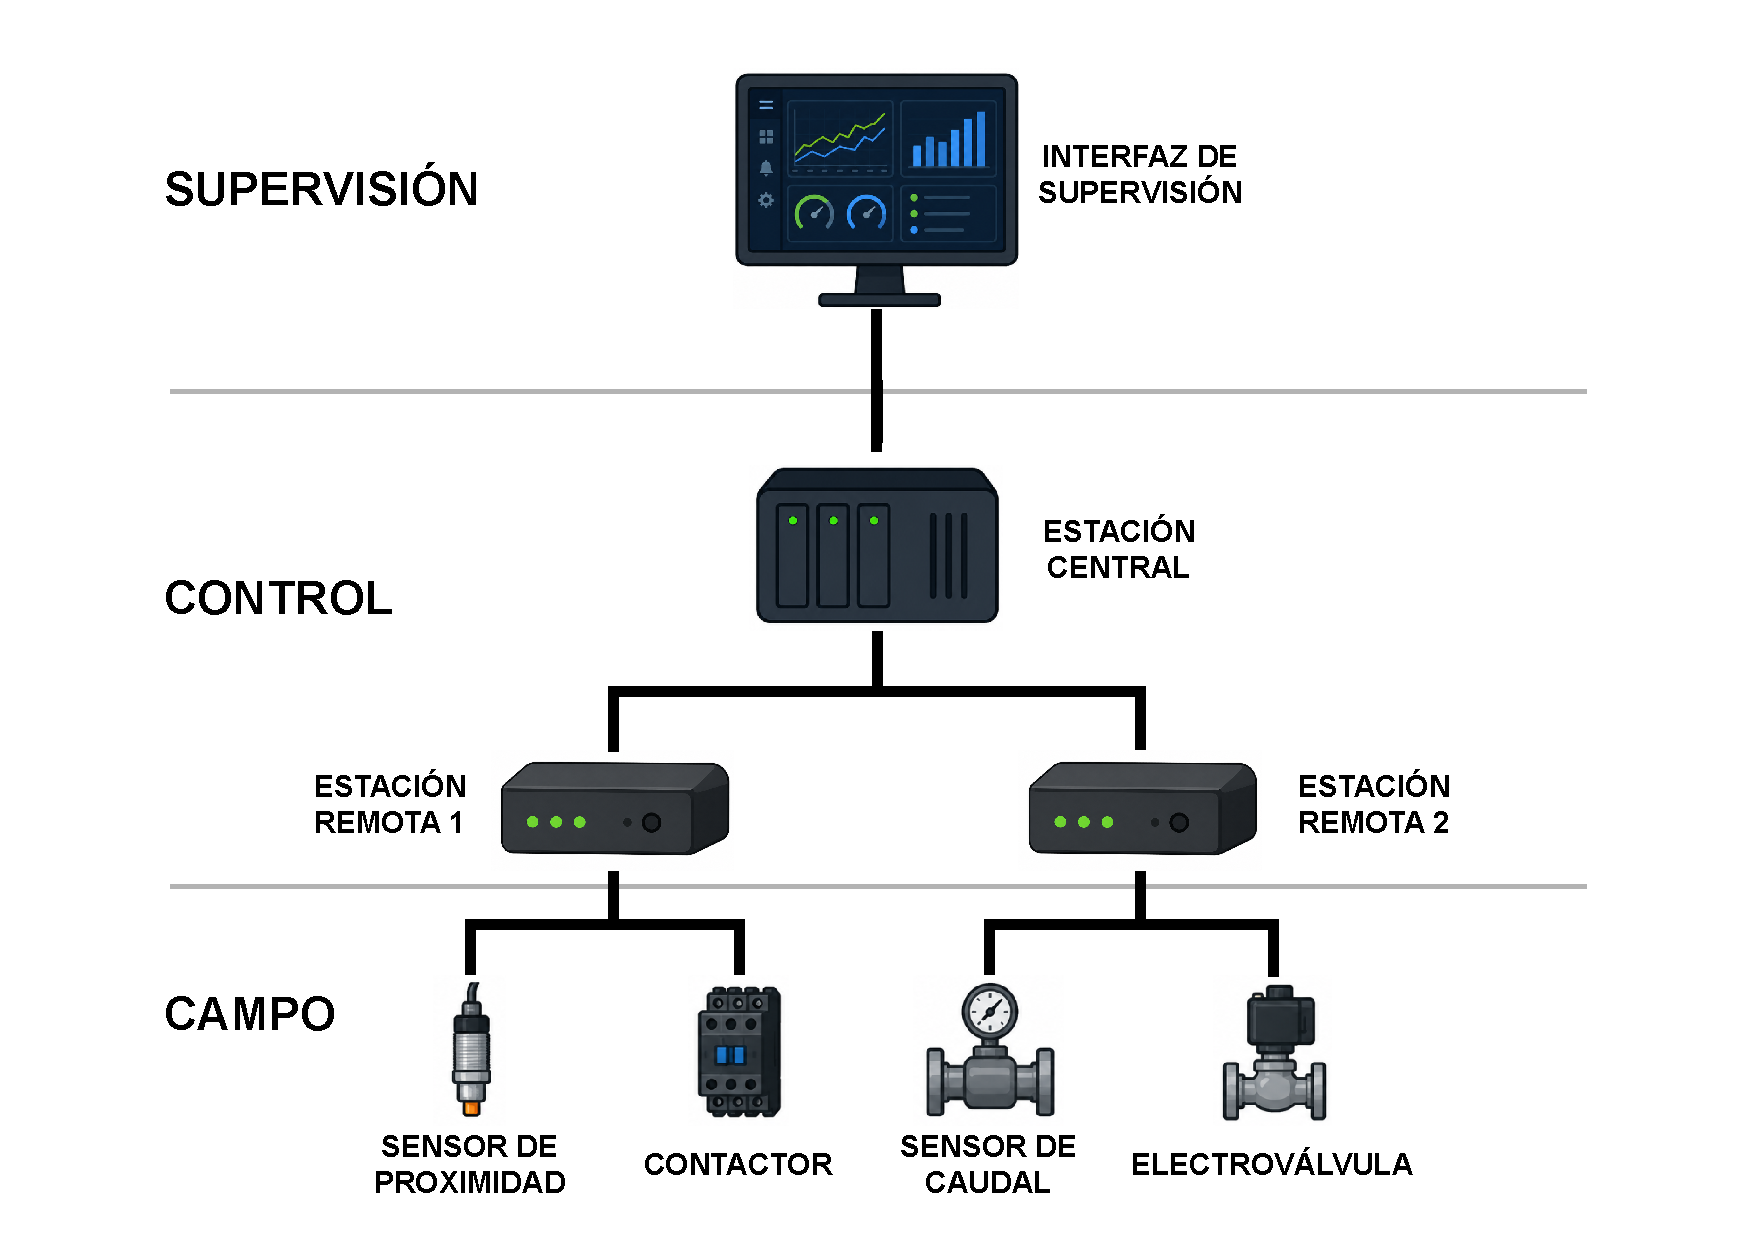
\includegraphics[scale=.4]{./Figures/red_control_distribuida.pdf}
	\caption{Arquitectura de un sistema distribuido de monitoreo y control industrial.}
	\label{fig:red_control_distribuida}
\end{figure}

%----------------------------------------------------------------------------------------

\section{Contexto y motivación}

Tradicionalmente, gran parte de los sistemas de automatización industrial se implementaron mediante arquitecturas centralizadas y redes cableadas. Si bien estas soluciones ofrecen altos niveles de robustez y confiabilidad, también presentan limitaciones en entornos donde el tendido de cables resulta costoso, complejo o poco práctico \cite{review_iwn_industry40}. Esta situación es frecuente en pequeñas y medianas industrias, instalaciones distribuidas geográficamente o procesos que requieren modificaciones frecuentes en la disposición física de los equipos.

En estos escenarios, la incorporación de tecnologías de comunicación inalámbrica permite aumentar la flexibilidad de instalación y reducir significativamente los costos asociados a infraestructura \cite{review_iwn_industry40}. Además, las arquitecturas distribuidas facilitan la expansión del sistema mediante la incorporación de nuevos nodos sin necesidad de realizar modificaciones importantes en el cableado existente.

Dentro de este contexto, los sistemas distribuidos de monitoreo y control representan una alternativa de creciente interés para aplicaciones industriales. Estas arquitecturas se basan en la utilización de una estación central y múltiples nodos remotos capaces de interactuar con sensores y actuadores ubicados en distintos puntos de una planta o instalación \cite{review_iwn_industry40}. La información recolectada puede transmitirse hacia sistemas de supervisión o control, lo que permite centralizar el monitoreo del proceso y mejorar la capacidad de diagnóstico y mantenimiento.

La motivación principal del presente trabajo surge de la necesidad de desarrollar una plataforma embebida flexible, escalable y de bajo costo de implementación, orientada a aplicaciones de monitoreo y control industrial distribuido. El sistema propuesto busca integrar capacidades de adquisición de señales, control de entradas y salidas, procesamiento local y comunicación entre nodos, utilizando una arquitectura modular que facilite su adaptación a diferentes escenarios de aplicación \cite{overview_embedded_i40}. Particularmente, se busca ofrecer una solución técnicamente viable para pequeñas y medianas industrias, donde los costos asociados a infraestructura y expansión suelen representar una limitación significativa para la incorporación de tecnologías de automatización.

%----------------------------------------------------------------------------------------

\section{Estado del arte}

La evolución de los sistemas de automatización industrial dio lugar al desarrollo de diversas tecnologías de comunicación destinadas a satisfacer los requerimientos de monitoreo y control de los procesos productivos. En la actualidad conviven soluciones cableadas e inalámbricas, cada una con características particulares en términos de desempeño, flexibilidad y costo de implementación. A continuación, se revisan las tecnologías más representativas relacionadas con la propuesta desarrollada en el presente trabajo.

\subsection{Redes industriales cableadas}

En los entornos de automatización industrial modernos, las redes de comunicación constituyen un elemento fundamental para la adquisición de datos, supervisión y control de procesos. Tradicionalmente, la industria ha adoptado soluciones cableadas debido a su elevada confiabilidad, inmunidad al ruido electromagnético y capacidad para garantizar tiempos de comunicación determinísticos \cite{future_industrial_communication,communication_technology_i40}.

Las redes industriales cableadas permiten la interconexión de sensores, actuadores, PLC (\textit{Programmable Logic Controller}, Controlador Lógico Programable) y sistemas de supervisión industrial, lo que posibilita el intercambio de información en tiempo real dentro de plantas y procesos automatizados. Entre las tecnologías más utilizadas se destacan buses de campo y soluciones basadas en Ethernet industrial, como PROFIBUS y PROFINET, ampliamente adoptadas en aplicaciones de automatización industrial \cite{profibus_official,profinet_official}.

La evolución de los sistemas industriales y la aparición de los conceptos de Industria 4.0 e IIoT (\textit{Industrial Internet of Things}, Internet Industrial de las Cosas) impulsaron además la integración de infraestructuras Ethernet, sistemas distribuidos y arquitecturas orientadas a comunicaciones en tiempo real \cite{future_industrial_communication}. Sin embargo, a pesar de sus ventajas en términos de robustez y desempeño, las soluciones cableadas presentan limitaciones asociadas a los costos de instalación, mantenimiento y expansión de infraestructura física, especialmente en aplicaciones distribuidas, móviles o de difícil acceso.

\subsection{Redes industriales inalámbricas}

En los últimos años, el avance de los conceptos de Industria 4.0 e IIoT impulsó el crecimiento de las redes inalámbricas industriales como complemento de las infraestructuras cableadas tradicionales \cite{review_iwn_industry40}. Estas tecnologías permiten reducir costos de instalación, simplificar tareas de mantenimiento y aumentar la flexibilidad de despliegue \cite{emerson_wireless,phoenix_trusted_wireless,scalance_wireless}.

Las redes inalámbricas industriales resultan particularmente atractivas para aplicaciones de monitoreo, adquisición distribuida de datos y automatización, debido a ventajas como la movilidad, la facilidad de expansión y la reducción del cableado físico \cite{review_iwn_industry40}. No obstante, los entornos industriales presentan desafíos significativos asociados a interferencias electromagnéticas, obstáculos físicos, topologías dinámicas y requisitos estrictos de latencia y confiabilidad, lo que impone exigencias adicionales sobre los protocolos de comunicación inalámbrica \cite{review_iwn_industry40}.

Gran parte de las soluciones inalámbricas industriales modernas \cite{wirelesshart_official,isa_official,zigbee_official} se basan en el estándar IEEE 802.15.4 \cite{ieee_standard}. Dicho estándar define las capas física PHY (\textit{Physical Layer}) y de control de acceso al medio MAC (\textit{Medium Access Control}) para redes inalámbricas personales de baja velocidad LR-WPAN (\textit{Low-Rate Wireless Personal Area Network}, Red Inalámbrica Personal de Baja Velocidad) \cite{ieee_standard}. Este estándar se caracteriza por su bajo consumo energético, baja complejidad y reducido costo de implementación, características que favorecieron su adopción en sistemas embebidos, redes de sensores inalámbricos e IoT (\textit{Internet of Things}, Internet de las Cosas) \cite{overview_embedded_i40}. Asimismo, múltiples protocolos industriales inalámbricos utilizan IEEE 802.15.4 como base tecnológica para la implementación de mecanismos de comunicación orientados a monitoreo y automatización industrial.

\subsection{Protocolos inalámbricos basados en IEEE 802.15.4}

Entre los protocolos inalámbricos industriales más difundidos basados en IEEE 802.15.4 se encuentra WirelessHART \cite{wirelesshart_official}, ampliamente utilizado en automatización de procesos. Este protocolo incorpora topologías de red mallada (mesh), mecanismos redundantes de comunicación y sincronización temporal, lo que permite aumentar la confiabilidad de la red frente a interferencias o fallas de enlace.

Otra tecnología relevante es ISA100.11a \cite{isa_official,review_iwn_industry40}, diseñada específicamente para aplicaciones industriales de monitoreo y control inalámbrico, con foco en interoperabilidad, escalabilidad y coexistencia con otras tecnologías de comunicación \cite{review_iwn_industry40}.

Zigbee \cite{zigbee_official,review_iwn_industry40} representa otra de las implementaciones más conocidas sobre IEEE 802.15.4. Aunque su adopción se concentra principalmente en aplicaciones IoT, domótica y monitoreo de bajo consumo, muchas de sus características técnicas, como el bajo costo, el soporte para topologías mesh y el reducido consumo energético, lo convierten en una referencia importante dentro del ecosistema de redes inalámbricas embebidas \cite{review_iwn_industry40}.

\subsection{Comparación de soluciones existentes}
La tabla \ref{tab:comparacion_tecnologias} presenta una comparación general entre algunas de las principales tecnologías de comunicación industrial utilizadas en aplicaciones de automatización y monitoreo. Se consideran características relacionadas con el medio de transmisión, las capacidades de tiempo real, el modelo de licenciamiento y el costo de implementación, incluyendo además la propuesta desarrollada en el presente trabajo.

\begin{table}[h]
	\centering
	\caption[Comparación de tecnologías industriales]{Comparación de tecnologías industriales.}
	\begin{tabular}{l c c c c}
		\toprule
		\textbf{Tecnología} & \textbf{Medio} & \textbf{T. real} & \textbf{Licencia} & \textbf{Costo} \\
		\midrule
		PROFIBUS \cite{profibus_official} & Cableado & Alto & Propietaria & Alto \\
		
		PROFINET \cite{profinet_official} & Cableado & Muy alto & Propietaria & Alto \\
		
		WirelessHART \cite{wirelesshart_official} & Inalámbrico & Medio & Requerida & Alto \\
		
		ISA100.11a \cite{isa_official} & Inalámbrico & Medio & Requerida & Alto \\
		
		Zigbee \cite{zigbee_official} & Inalámbrico & Bajo & Parcialmente abierta & Medio \\
		
		Propuesta & Inalámbrico & Medio & Propia & Bajo \\
		\bottomrule
		\hline
	\end{tabular}
	\label{tab:comparacion_tecnologias}
\end{table}

La solución propuesta en este trabajo toma como referencia las arquitecturas inalámbricas industriales modernas basadas en IEEE 802.15.4, priorizando una implementación flexible, modular y de bajo costo orientada a aplicaciones embebidas de monitoreo y control distribuido. El desarrollo busca proporcionar una plataforma adaptable a distintos procesos productivos, capaz de integrarse con sensores y actuadores industriales mediante una arquitectura escalable y reutilizable. Asimismo, se plantea como una alternativa de bajo costo de implementación orientada a pequeñas y medianas industrias, donde las limitaciones económicas y de infraestructura suelen dificultar la incorporación de soluciones convencionales de automatización industrial.

%----------------------------------------------------------------------------------------

\section{Objetivos del trabajo}

Los objetivos definidos para el presente trabajo establecen el propósito general del sistema desarrollado y delimitan las principales actividades necesarias para su diseño, implementación y validación. A continuación, se presentan el objetivo general y los objetivos específicos que guiaron el desarrollo del proyecto.

\subsection{Objetivo general}
Desarrollar un sistema embebido modular y escalable orientado a aplicaciones de monitoreo y control industrial distribuido, basado en una arquitectura compuesta por una estación central y múltiples estaciones remotas interconectadas mediante comunicación inalámbrica \cite{proyecto}.

\subsection{Objetivos específicos}
Los objetivos específicos definidos para el desarrollo del presente trabajo son los siguientes \cite{proyecto}:

\begin{itemize}
	\item Diseñar e implementar un prototipo funcional de estación central basado en un microcontrolador de altas prestaciones capaz de ejecutar un sistema operativo de tiempo real RTOS (\textit{Real-Time Operating System}, Sistema Operativo de Tiempo Real).
	
	\item Diseñar e implementar prototipos funcionales de estaciones remotas con capacidad de adquisición de señales y control de entradas y salidas industriales.
	
	\item Implementar un sistema de comunicación inalámbrica entre estaciones utilizando tecnología basada en IEEE 802.15.4.
	
	\item Desarrollar el firmware necesario para la inicialización y gestión de periféricos, comunicaciones y manejo de entradas y salidas en las estaciones central y remotas.
	
	\item Diseñar una arquitectura de software modular que permita abstraer las dependencias de hardware y facilite la reutilización y escalabilidad del sistema.
	
	\item Implementar interfaces de conexión para sensores y actuadores industriales que permitan adaptar el sistema a diferentes aplicaciones de monitoreo y control.
	
	\item Diseñar e implementar la arquitectura de alimentación de las estaciones.
	
	\item Validar el funcionamiento del sistema mediante pruebas experimentales orientadas a verificar la comunicación entre nodos, el procesamiento de señales y el control de entradas y salidas.
	
\end{itemize}

\chapter{Introducción específica}
\label{Chapter2}

En este capítulo se describen las principales plataformas de hardware, componentes externos, capas de software y protocolos de comunicación utilizados durante el desarrollo del trabajo. Asimismo, se presentan las tecnologías de terceros empleadas para la implementación de las funciones de adquisición, procesamiento y comunicación del sistema.

%----------------------------------------------------------------------------------------

\section{Plataforma de hardware}

Tanto la estación central como las estaciones remotas del sistema utilizan el microcontrolador STM32H563RI de STMicroelectronics, perteneciente a la familia STM32H5 \cite{STM32H563,STMicroelectronics,STM32H5}. Esta decisión permitió uniformar la arquitectura de hardware y simplificar el desarrollo y mantenimiento del firmware. Además, facilitó la reutilización de controladores, configuraciones de periféricos y capas de abstracción de hardware entre ambos tipos de nodos.

El STM32H563RI se basa en una arquitectura ARM Cortex-M33 de 32 bits \cite{CortexM33}, orientada a sistemas embebidos de alto rendimiento y plataformas conectadas. El núcleo incorpora una unidad de punto flotante FPU (\textit{Floating Point Unit}, Unidad de Punto Flotante), extensiones DSP (\textit{Digital Signal Processing}, Procesamiento Digital de Señales) y mecanismos de seguridad basados en TrustZone \cite{STM32H5,STM32H563_RefManual}, adecuados para aplicaciones industriales e IoT.

El microcontrolador dispone de memoria Flash integrada y memoria SRAM (\textit{Static Random Access Memory}, Memoria Estática de Acceso Aleatorio) interna, además de una amplia variedad de periféricos de comunicación y control \cite{STM32H563}. Entre los periféricos utilizados durante el desarrollo se encuentran interfaces SPI (\textit{Serial Peripheral Interface}, Interfaz Periférica Serie), UART (\textit{Universal Asynchronous Receiver-Transmitter}, Transmisor-Receptor Asíncrono Universal) y Ethernet MAC (\textit{Media Access Control}, Control de Acceso al Medio).

La selección de este microcontrolador también se fundamentó en la disponibilidad de herramientas de desarrollo y middleware provistos por STMicroelectronics, incluyendo STM32CubeIDE \cite{stm32cubeide}, bibliotecas HAL (\textit{Hardware Abstraction Layer}, Capa de Abstracción de Hardware) \cite{hal} y soporte para sistemas operativos de tiempo real como FreeRTOS (\textit{Free Real-Time Operating System}, Sistema Operativo de Tiempo Real Libre) \cite{freertos}. Estas herramientas simplificaron significativamente el desarrollo, depuración y mantenimiento del firmware del sistema.

%----------------------------------------------------------------------------------------

\section{Componentes y módulos externos}

Complementariamente a la plataforma de procesamiento basada en el STM32H563RI, el sistema incorpora distintos circuitos integrados y módulos externos orientados a la adquisición de señales industriales, manejo de salidas, comunicación cableada e inalámbrica y validación del firmware durante las etapas de desarrollo. A continuación, se describen los componentes más relevantes utilizados en el trabajo.

\subsection{SCLT3-8BT8}

El SCLT3-8BT8 de STMicroelectronics es una interfaz de entradas digitales industriales de ocho canales con transferencia serializada de estados mediante interfaz SPI \cite{sclt38bt8}. El dispositivo está orientado a aplicaciones de automatización industrial y PLC. Además, proporciona adaptación y protección para señales de 24 V provenientes de sensores y dispositivos industriales.

El circuito incorpora protección contra sobretensiones y compatibilidad con estándares industriales de inmunidad electromagnética, incluyendo IEC61000-4-2, IEC61000-4-4 e IEC61000-4-5. Además, dispone de indicadores de estado integrados y mecanismos de diagnóstico para detección de fallas en las entradas.

\subsection{VNI8200XP-32}

El VNI8200XP-32 de STMicroelectronics es un controlador de salidas digitales industriales de ocho canales basado en transistores MOSFET (\textit{Metal-Oxide-Semiconductor Field-Effect Transistor}, Transistor de Efecto de Campo Metal-Óxido-Semiconductor) de tipo \textit{high-side} \cite{vni8200xp32}. El dispositivo permite accionar cargas industriales de 24 V mediante una interfaz SPI o paralelo configurable.

El componente incorpora funciones de protección y diagnóstico, incluyendo protección térmica, limitación de corriente, detección de sobrecorriente, monitoreo de alimentación y señalización de fallas. También dispone de mecanismos específicos frente a condiciones de cortocircuito y sobretemperatura, características relevantes en aplicaciones industriales.

\subsection{SN65HVD82}

El SN65HVD82 de Texas Instruments es un transceptor RS-485 (\textit{Recommended Standard 485}, Estándar de Comunicación Diferencial Serie) diseñado para comunicaciones industriales robustas \cite{sn65hvd82}. El dispositivo opera con alimentación de 5 V y proporciona transmisión diferencial compatible con buses multipunto de larga distancia.

El componente incorpora protección ESD (\textit{Electrostatic Discharge}, Descarga Electrostática) conforme a normas IEC orientadas a aplicaciones industriales y permite operación en entornos con elevado nivel de ruido electromagnético. Además, soporta altas velocidades de transmisión y presenta bajo consumo energético.

\subsection{MRF24J40}

El MRF24J40 de Microchip es un transceptor inalámbrico compatible con el estándar IEEE 802.15.4 \cite{mrf24j40}. El dispositivo opera en la banda ISM (\textit{Industrial, Scientific and Medical}, Industrial, Científica y Médica) de 2.4 GHz y está orientado a aplicaciones de redes inalámbricas de bajo consumo.

El componente incorpora las capas PHY y MAC, además de mecanismos de cifrado AES-128 (\textit{Advanced Encryption Standard}, Estándar de Cifrado Avanzado). La comunicación con el microcontrolador se realiza mediante interfaz SPI.

\subsection{LAN8742A}

El LAN8742A de Microchip es un transceptor Ethernet PHY compatible con Ethernet 10BASE-T y 100BASE-TX \cite{lan8742a}. El dispositivo se comunica con el microcontrolador mediante interfaz RMII (\textit{Reduced Media Independent Interface}, Interfaz Independiente del Medio Reducida), lo que permite implementar conectividad Ethernet de bajo número de pines.

El componente incorpora soporte para auto-negociación, detección automática de polaridad y tecnología HP Auto-MDIX (\textit{Automatic Medium-Dependent Interface Crossover}, Cruce Automático de Interfaz Dependiente del Medio), característica que permite utilizar cables directos o cruzados. Además, dispone de mecanismos de administración de energía y soporte para Wake-on-LAN (\textit{Wake on Local Area Network}, Activación mediante Red Local).

\subsection{Kits de desarrollo y evaluación}

Durante las etapas iniciales del proyecto se utilizaron placas STM32 NUCLEO-H563ZI \cite{nucleoh563}, basadas en el microcontrolador STM32H563ZI. Estas placas permitieron realizar pruebas funcionales y tareas de depuración temprana antes del desarrollo del hardware definitivo.

Asimismo, se empleó la placa de expansión X-NUCLEO-PLC01A1 \cite{nucleoplc}, orientada a aplicaciones PLC industriales. Esta placa integra los dispositivos SCLT3-8BT8 \cite{sclt38bt8} y VNI8200XP-32 \cite{vni8200xp32}, que proporcionan entradas y salidas industriales de 24 V manejadas mediante SPI. Su utilización permitió validar la arquitectura de firmware y los controladores desarrollados para las interfaces industriales utilizadas posteriormente en el diseño final.

%----------------------------------------------------------------------------------------

\section{Sistema operativo y middleware}

El desarrollo del firmware del sistema se realizó utilizando distintas capas de software orientadas a facilitar la abstracción del hardware, la administración de tareas concurrentes y la implementación de protocolos de comunicación.

\subsection{FreeRTOS}

FreeRTOS es un sistema operativo de tiempo real orientado a sistemas embebidos \cite{freertos}. El sistema proporciona mecanismos de planificación multitarea basados en prioridades, sincronización mediante semáforos y mutex, comunicación entre tareas y administración de temporizadores de software.

La utilización de un RTOS permitió implementar múltiples tareas concurrentes asociadas a adquisición de datos, comunicación inalámbrica y procesamiento de protocolos Ethernet. FreeRTOS también facilitó la modularización del firmware y la separación funcional entre los distintos subsistemas de la aplicación.

\subsection{HAL y BSP}

Para el acceso y configuración de los periféricos del microcontrolador se utilizaron las bibliotecas HAL (\textit{Hardware Abstraction Layer}, Capa de Abstracción de Hardware) y BSP (\textit{Board Support Package}, Paquete de Soporte de Placa) provistas por STMicroelectronics \cite{hal,bsp}.

La capa HAL proporciona funciones de alto nivel para el manejo de periféricos internos del microcontrolador, incluyendo interfaces SPI, UART, Ethernet y temporizadores. Esta capa simplifica el desarrollo del firmware mediante una interfaz uniforme e independiente de registros específicos del hardware.

Por otro lado, la capa BSP incorpora controladores y configuraciones específicas para placas de desarrollo y módulos de evaluación utilizados durante el proyecto, facilitando la inicialización y utilización de periféricos externos integrados en dichas plataformas.

\subsection{lwIP}

Para la implementación de conectividad Ethernet y protocolos TCP/IP (\textit{Transmission Control Protocol/Internet Protocol}, Protocolo de Control de Transmisión/Protocolo de Internet) se utilizó el \textit{stack} lwIP (\textit{Lightweight IP}) \cite{tcpip,lwip}.

lwIP es una implementación liviana del protocolo TCP/IP \cite{tcpip} orientada a sistemas embebidos con recursos limitados. El \textit{stack} incorpora soporte para protocolos IPv4, TCP, UDP (\textit{User Datagram Protocol}, Protocolo de Datagrama de Usuario), ICMP (\textit{Internet Control Message Protocol}, Protocolo de Mensajes de Control de Internet), DHCP (\textit{Dynamic Host Configuration Protocol}, Protocolo de Configuración Dinámica de Host) y ARP (\textit{Address Resolution Protocol}, Protocolo de Resolución de Direcciones).

En el sistema desarrollado, lwIP fue integrado junto con FreeRTOS y el periférico Ethernet del STM32H563RI. Esta integración permitió implementar comunicación Ethernet para supervisión, configuración y transmisión de datos mediante redes TCP/IP.

\section{Protocolos e interfaces de comunicación}

El sistema desarrollado utiliza distintas interfaces y protocolos de comunicación orientados a la adquisición de datos, control de periféricos, conectividad Ethernet y depuración del firmware. La selección de cada interfaz se realizó en función de los requerimientos de velocidad, complejidad de implementación, robustez y compatibilidad con los dispositivos externos utilizados en el proyecto.

\subsection{SPI}

La interfaz SPI fue utilizada para la comunicación entre el microcontrolador y distintos circuitos integrados externos, incluyendo las interfaces industriales SCLT3-8BT8 \cite{sclt38bt8} y VNI8200XP-32 \cite{vni8200xp32}, así como también el transceptor inalámbrico MRF24J40 \cite{mrf24j40}.

SPI es un protocolo de comunicación serial síncrono basado en una arquitectura maestro-esclavo, caracterizado por su elevada velocidad de transferencia y baja complejidad de implementación. La interfaz utiliza líneas dedicadas de transmisión, recepción y señal de reloj, además de señales independientes de selección de dispositivo.

\subsection{UART y RS-485}

La interfaz UART fue utilizada junto con el transceptor SN65HVD82 \cite{sn65hvd82} para implementar comunicación RS-485 (\textit{Recommended Standard 485}, Estándar de Comunicación Diferencial Serie) \cite{rs485}.

UART permite establecer comunicaciones seriales asíncronas mediante transmisión y recepción de datos sin necesidad de señal de reloj compartida. En conjunto con RS-485, posibilita implementar enlaces diferenciales robustos, adecuados para entornos industriales con elevado nivel de ruido electromagnético y largas distancias de cableado.

\subsection{Ethernet y RMII}

La conectividad Ethernet del sistema se implementó mediante el periférico Ethernet MAC integrado en el microcontrolador STM32H563RI \cite{STM32H563_RefManual} y el transceptor Ethernet PHY LAN8742A \cite{lan8742a}.

La comunicación entre el microcontrolador y el PHY se realizó mediante la interfaz RMII (\textit{Reduced Media Independent Interface}, Interfaz Independiente del Medio Reducida) \cite{rmii}, utilizada para transmisión y recepción de datos Ethernet con bajo número de pines.

La capa física Ethernet permite establecer comunicación 10BASE-T y 100BASE-TX sobre medio cableado de par trenzado. Esto facilita la integración con redes Ethernet industriales y servicios basados en TCP/IP.

\subsection{GPIO}

Las interfaces GPIO (\textit{General Purpose Input/Output}, Entrada/Salida de Propósito General) fueron utilizadas para el manejo de señales digitales de control, monitoreo de estados y accionamiento de indicadores luminosos.

Estas señales incluyen líneas de habilitación de periféricos, señales de interrupción, selección de dispositivos SPI, monitoreo de estados de alimentación y control de LEDs indicadores presentes en la placa.

\subsection{SWD}

La programación y depuración del microcontrolador se realizó mediante la interfaz SWD (\textit{Serial Wire Debug}, Depuración Serie de Dos Hilos) \cite{swi}, utilizada por las herramientas de desarrollo STMicroelectronics.

SWD constituye una interfaz de depuración derivada de JTAG (\textit{Joint Test Action Group}) \cite{jtag}. Esta interfaz reduce la cantidad de señales requeridas y conserva capacidades de programación, ejecución paso a paso, lectura de memoria y monitoreo interno del sistema embebido.
\chapter{Diseño e implementación}
\label{Chapter3}

En el presente capítulo se describe el diseño e implementación del sistema desarrollado. Se presentan la arquitectura general de hardware y software, los criterios utilizados para la selección de componentes y las principales decisiones de diseño adoptadas durante el desarrollo. Asimismo, se detallan la estructura del firmware, las comunicaciones implementadas y la integración entre los distintos módulos del sistema.

%----------------------------------------------------------------------------------------
\section{Arquitectura del sistema}
La figura \ref{fig:arquitectura_general} presenta la arquitectura general del sistema desarrollado. La solución se compone de una estación central conectada mediante Ethernet TCP/IP a la interfaz de usuario y múltiples estaciones remotas enlazadas de forma inalámbrica mediante IEEE 802.15.4. Cada estación remota interactúa con variables de proceso asociadas a sensores, actuadores e interfaces industriales.

\begin{figure}[ht]
	\centering
	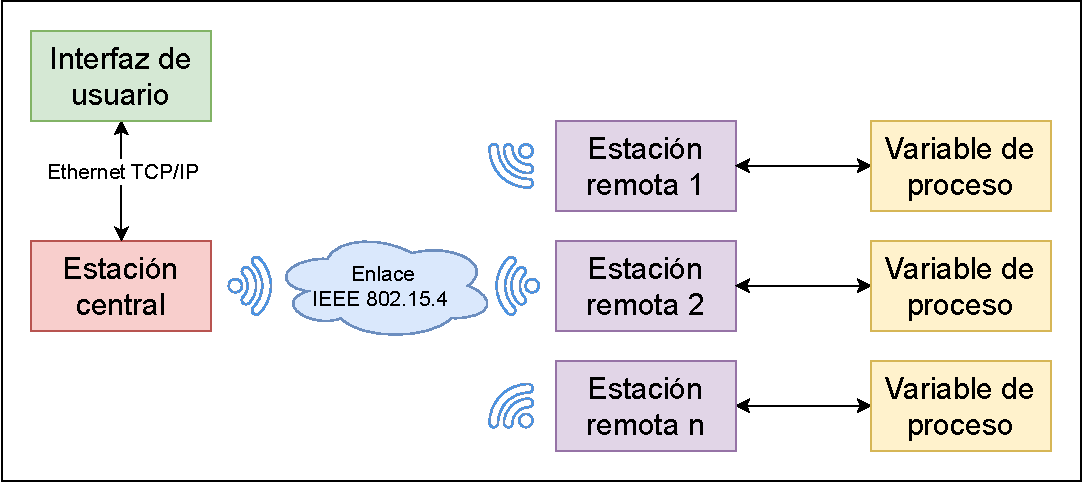
\includegraphics[width=1.0\textwidth]{./Figures/arquitectura_general.pdf}
	\caption{Arquitectura general del sistema implementado.}
	\label{fig:arquitectura_general}
\end{figure}

\subsection{Diagrama de bloques del hardware}

La figura \ref{fig:arquitectura_hardware} presenta el diagrama de bloques del hardware desarrollado. La arquitectura se basa en un microcontrolador encargado de gestionar las interfaces de comunicación, las entradas y salidas industriales y los módulos auxiliares del sistema. Asimismo, se distinguen los bloques comunes a las estaciones centrales y remotas y aquellos específicos de cada tipo de nodo.

Con el objetivo de uniformar el desarrollo y reducir costos durante una etapa inicial del trabajo, se implementó un único diseño de placa de circuito impreso PCB (\textit{Printed Circuit Board}, Placa de Circuito Impreso) tanto para las estaciones centrales como para las estaciones remotas. Esta estrategia permitió reutilizar el mismo diseño base de hardware y poblar únicamente los componentes requeridos según las funcionalidades de cada estación. Además de simplificar el proceso de desarrollo, esta decisión redujo los costos de fabricación y facilitó las tareas de validación y mantenimiento del sistema.

La estación central incorpora un transceptor Ethernet para la comunicación con una interfaz de usuario ubicada en un nivel jerárquico superior. Asimismo, dispone de un reloj de tiempo real RTC (\textit{Real-Time Clock}, Reloj de Tiempo Real), utilizado para el registro y mantenimiento de fecha y hora ante interrupciones en la alimentación principal.

Por otro lado, las estaciones remotas incorporan una interfaz RS485 para la comunicación con instrumentos industriales y módulos de entradas y salidas digitales destinados a la adquisición y accionamiento de variables de proceso.

Tanto las estaciones centrales como las remotas comparten los módulos de alimentación y regulación de tensión, el microcontrolador principal y el transceptor inalámbrico IEEE 802.15.4 utilizado para la comunicación entre nodos.

\begin{figure}[ht]
	\centering
	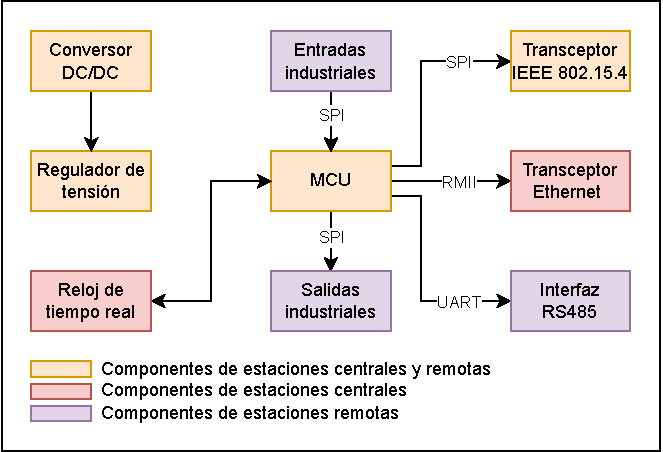
\includegraphics[width=1.0\textwidth]{./Figures/arquitectura_hardware.pdf}
	\caption{Diagrama de bloques general del hardware.}
	\label{fig:arquitectura_hardware}
\end{figure}

\subsection{Diagrama de bloques del firmware}
La figura \ref{fig:arquitectura_firmware} presenta la arquitectura general del firmware implementado en el sistema. Este fue organizado en capas con el objetivo de desacoplar la lógica de aplicación de las dependencias específicas del hardware y facilitar la reutilización de código entre estaciones centrales y remotas.

La capa superior contiene la lógica de control y supervisión del sistema. Por debajo se ubica una API (\textit{Application Programming Interface}, Interfaz de Programación de Aplicaciones) encargada de abstraer el acceso a sensores, actuadores e interfaces del sistema. Las capas intermedias incorporan los servicios de middleware, incluyendo el sistema operativo en tiempo real FreeRTOS y la pila de comunicaciones lwIP. Finalmente, las capas inferiores contienen los controladores de periféricos, la capa de abstracción de hardware HAL (\textit{Hardware Abstraction Layer}, Capa de Abstracción de Hardware) y los módulos físicos del sistema.

\begin{figure}[ht]
	\centering
	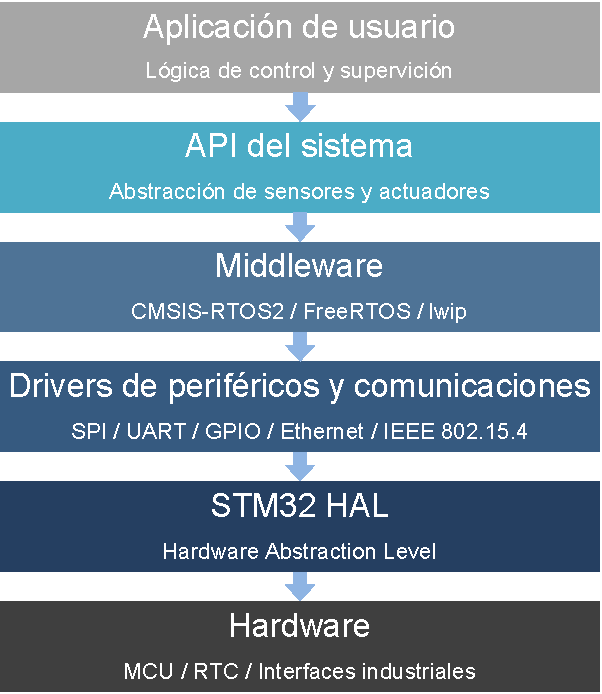
\includegraphics[width=0.7\textwidth]{./Figures/arquitectura_firmware.pdf}
	\caption{Diagrama de bloques general del firmware.}
	\label{fig:arquitectura_firmware}
\end{figure}

%\chapter{Ensayos y resultados}
\label{Chapter4}

En este capítulo se presentan los ensayos realizados para verificar el funcionamiento del hardware y firmware desarrollados, así como su integración en el sistema completo. Las pruebas comprenden la evaluación de los principales bloques de hardware, las funciones implementadas en el firmware y la comunicación entre la estación central y las estaciones remotas. Finalmente, se analizan los resultados obtenidos y los principales desvíos y limitaciones identificados durante la validación.

%----------------------------------------------------------------------------------------
\section{Plan de ensayos}

La validación del sistema se realizó siguiendo una metodología incremental, comenzando por la verificación individual de los distintos bloques de hardware y firmware y continuando con ensayos de integración entre ambos niveles. Finalmente, se consideran pruebas sobre el sistema completo, orientadas a comprobar el intercambio de información y la ejecución coordinada de las funciones implementadas entre la estación central y las estaciones remotas.

Para cada ensayo se establecieron las condiciones iniciales, la configuración utilizada, el procedimiento de prueba y los resultados esperados. Las pruebas de hardware se orientaron principalmente a verificar las etapas de alimentación, las entradas y salidas digitales y las interfaces de comunicación. Los ensayos de firmware contemplan la comprobación de los controladores y servicios desarrollados, la ejecución de las tareas de FreeRTOS y la temporización de las operaciones relevantes. Por último, las pruebas de integración evalúan el funcionamiento conjunto de estos elementos mediante operaciones representativas del sistema.

Los ensayos se realizaron en condiciones controladas de laboratorio empleando el instrumental y las herramientas de desarrollo indicados en la tabla \ref{tab:instrumental_ensayos}. Los criterios de aceptación se establecieron a partir de los requerimientos funcionales del sistema y de las especificaciones de los componentes utilizados. Según el tipo de ensayo, se consideraron los niveles de tensión y corriente, las características temporales de las señales, la correcta ejecución de las funciones y el intercambio de información entre los distintos módulos.

\begin{table}[H]
	\centering
	\caption[Instrumental y herramientas utilizados en los ensayos]
	{Instrumental y herramientas utilizados para la realización de los ensayos.}
	\begin{tabular}{l l}
		\toprule
		\textbf{Instrumento o herramienta} & \textbf{Utilización} \\
		\midrule
		Fuente regulada de laboratorio
		& Alimentación del sistema \\
		
		Multímetro digital
		& Medición de tensión y corriente \\
		
		Osciloscopio digital
		& Análisis temporal de señales \\
		
		Analizador lógico USB de 8 canales
		& Análisis de señales digitales \\
		
		Generador de señales digitales
		& Estimulación de entradas \\
		
		STLINK-V3MINIE
		& Programación y depuración \\
		
		STM32CubeIDE
		& Depuración del firmware \\
		
		Vistas de FreeRTOS
		& Supervisión de objetos del RTOS \\
		
		Interfaz SWO
		& Registro de eventos y variables \\
		
		Contador de ciclos DWT
		& Medición de tiempos de ejecución \\
		\bottomrule
	\end{tabular}
	\label{tab:instrumental_ensayos}
\end{table}

%----------------------------------------------------------------------------------------
\section{Ensayos de hardware}

En esta sección se presentan los ensayos realizados sobre los principales bloques de hardware del sistema. Las pruebas comprenden la verificación de las tensiones de alimentación y el consumo de corriente, el funcionamiento de las entradas y salidas digitales y las señales asociadas a las interfaces de comunicación. Para cada ensayo se indican las condiciones de medición y los resultados obtenidos mediante el instrumental presentado en la sección anterior.

%----------------------------------------------------------------------------------------
\subsection{Ensayo de las etapas de alimentación y consumo}

Como primera etapa de validación del hardware se verificaron las principales tensiones de alimentación y el consumo de corriente de la placa. El sistema se alimentó con 24 V y se midieron mediante un multímetro digital las líneas de 5 V y 3,3 V, junto con la corriente consumida desde la alimentación principal. Esta última medición se realizó con la placa en estado de reposo, sin cargas externas conectadas ni operaciones activas de adquisición, actuación o comunicación. Los valores obtenidos se presentan en la tabla \ref{tab:alimentacion_consumo}.

\begin{table}[h]
	\centering
	\caption[Mediciones de alimentación y consumo]{Mediciones de las tensiones de alimentación y del consumo de corriente de la placa.}
	\begin{tabular}{l c c}
		\toprule
		\textbf{Magnitud} & \textbf{Nominal} & \textbf{Medido} \\
		\midrule
		Alimentación de entrada & 24 V  & 24 V \\
		Alimentación de 5 V     & 5 V   & 5,02 V \\
		Alimentación de 3,3 V   & 3,3 V & 3,31 V \\
		Consumo a 24 V          & --    & 21 mA \\
		\bottomrule
	\end{tabular}
	\label{tab:alimentacion_consumo}
\end{table}

Los resultados obtenidos verifican el correcto funcionamiento de las etapas de alimentación en las condiciones consideradas, con niveles de 5 V y 3,3 V próximos a sus valores nominales y un consumo base de 21 mA sobre la alimentación de entrada de 24 V.
%\include{Chapters/Chapter5}

%----------------------------------------------------------------------------------------
% Apéndices
%----------------------------------------------------------------------------------------

\appendix

% Incluir apéndices desde archivos separados si es necesario
%\include{Appendices/AppendixA}

%----------------------------------------------------------------------------------------
% Bibliografía
%----------------------------------------------------------------------------------------

\renewcommand{\bibname}{Bibliografía} % Para asegurarte de que el título sea correcto
\phantomsection % Necesario para que el enlace del marcador sea correcto

\printbibliography[heading=bibintoc]

\end{document}






